\chapter{Fejlesztői dokumentáció} % Developer guide
\label{ch:impl}

\section{Tervezés}

\subsection{Kezdeti tervek}
Mivel egy játék (legyen akármekkora is) egy bonyolult rendszer, és mivel alapértelmezetten is egy jó gyakorlat, a projekt elejétől kezdve meg szerettem volna tervezni, átfogólag a különböző rendszereket. Tudtam előre, hogy a Unity játékmotort fogom használni a példajáték elkészítéséhez, és a tervminták alkalmazására, amiknek fontosságára Jason Weimann\cite{jason}, DapperDino\cite{dapperDino} és a Game Programming Patterns-ben\cite{gameProgrammingPatterns} olvasottak inspiráltak. Azt is figyelmemben tartottam, hogy szakdolgozatom célja a tervezési minták és programozási elvek felhasználása a játékfejlesztésben és egy nem feltétlenül teljes mértékben kidolgozott játék piacra dobása.\\*
Mindezek után három dolgot tartottam fontosnak eleinte, a játékos (és ellenségek) statemachine-ját, egy általánost leírás az alap rendszerek kapcsolatáról, valamint a játékom elkészítése a S.O.L.I.D elvek szerint.
\begin{figure}[H]
	\noindent\makebox[\textwidth]{
	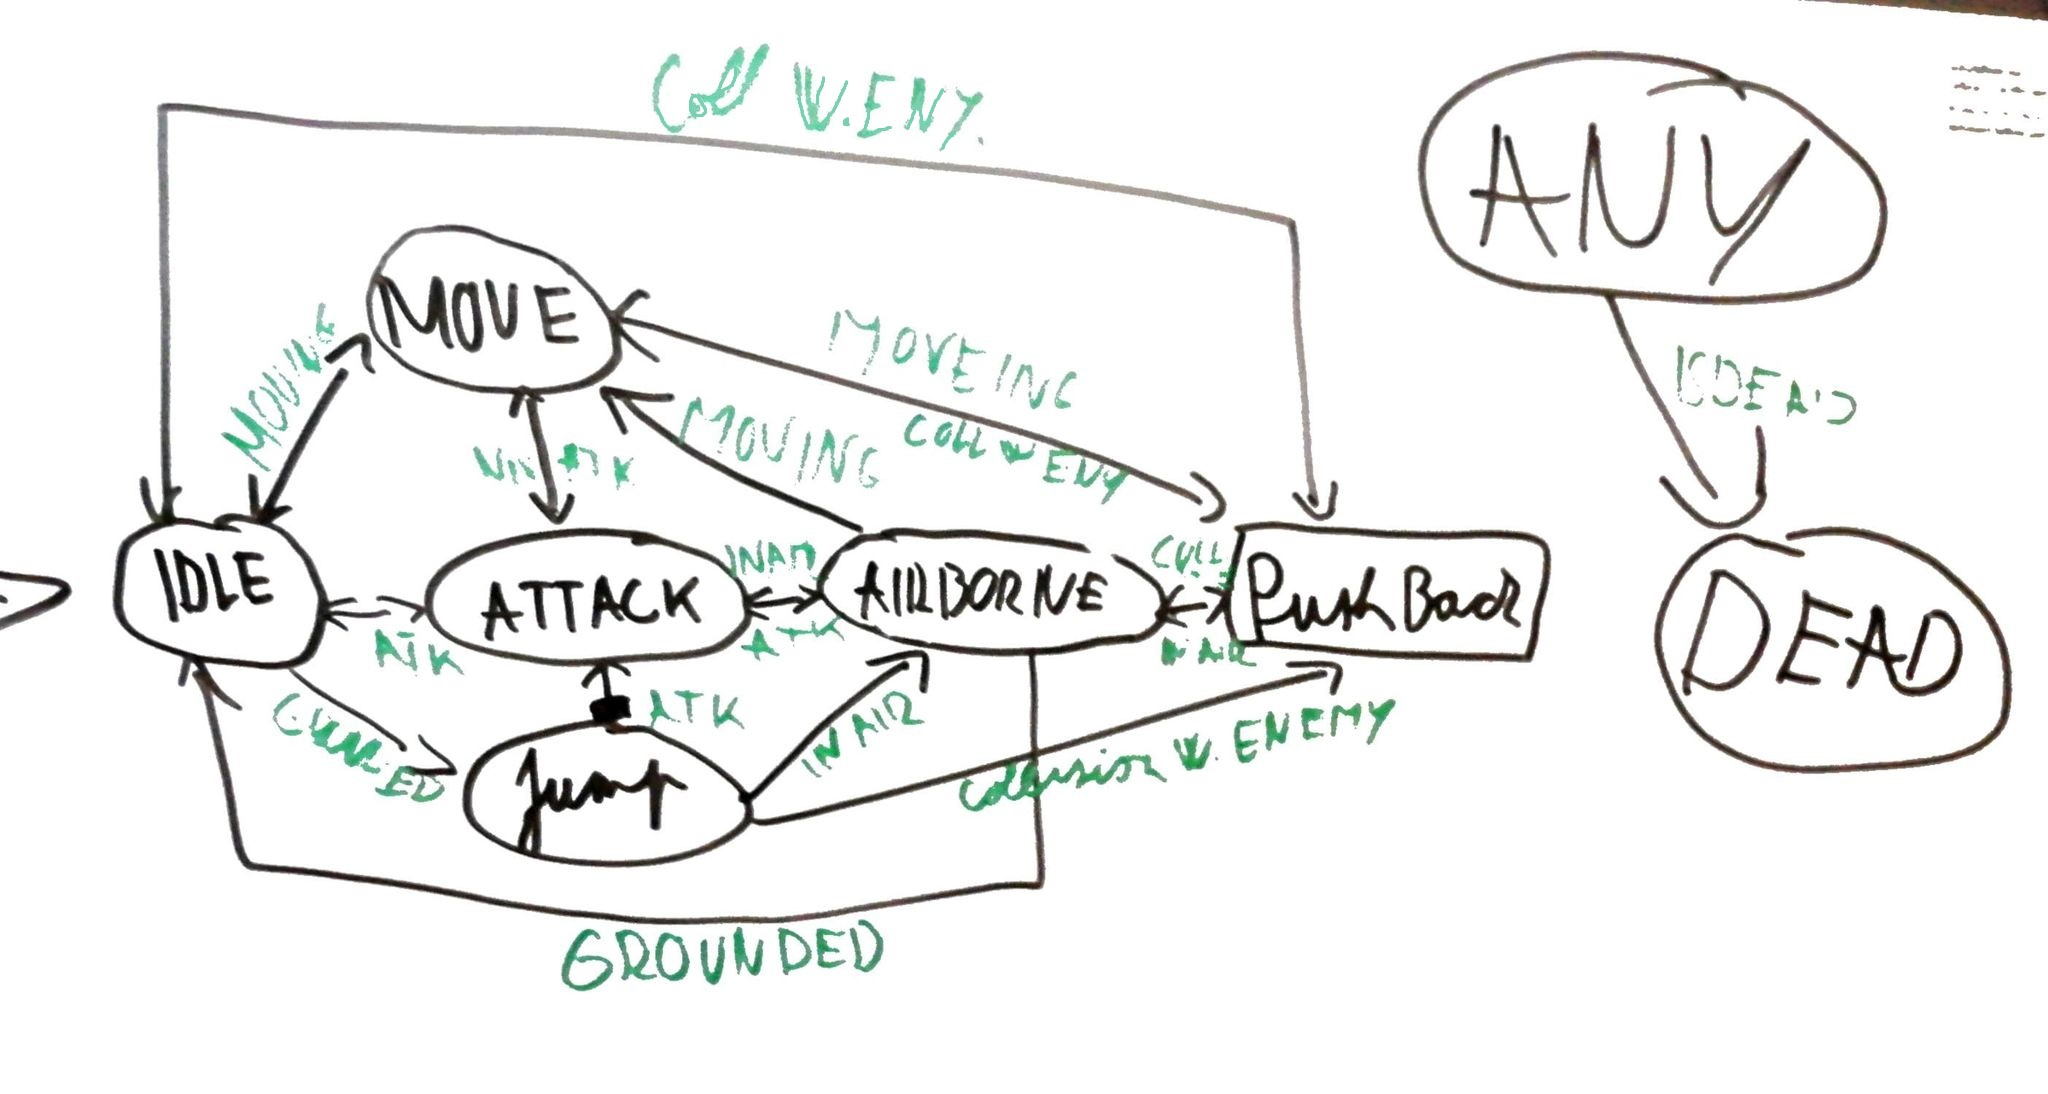
\includegraphics[width= 0.8\textwidth]{statemachine}}
	\caption{Kezdeti statemachine}
	\label{statemachine}
\end{figure}

\begin{figure}[H]
	\noindent\makebox[\textwidth]{
	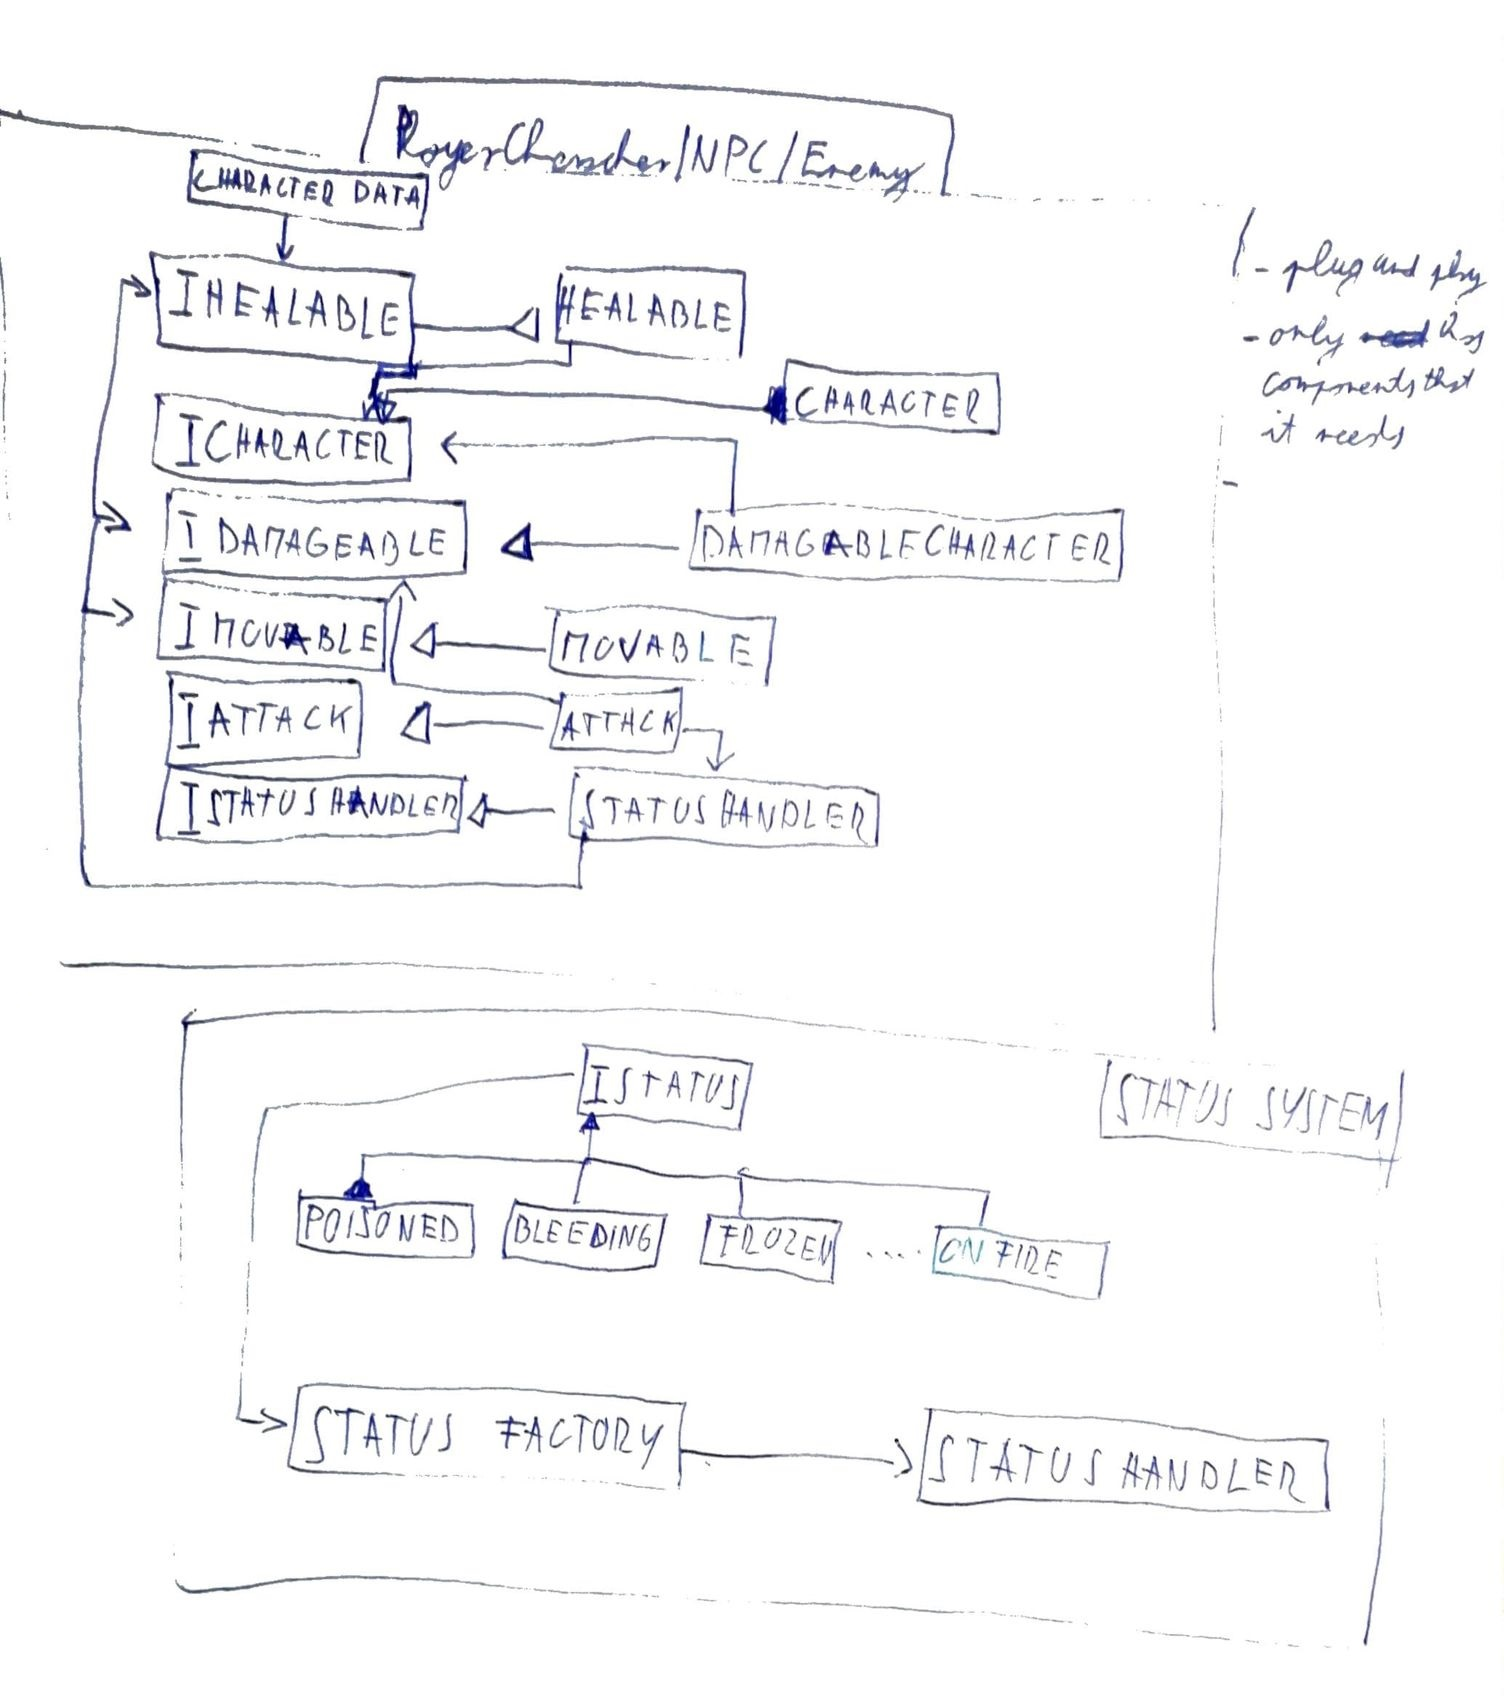
\includegraphics[width= 0.8\textwidth]{statussys}}
	\caption{Rendszerek általános leírása}
	\label{statussys}
\end{figure}

Azonban hamar rájöttem, hogy bizonyos bonyolultan rendszerek kapcsolatát érdemes jobban kifejteni. Ilyen volt a támadással foglalkozó csoport is, ahol három kisebb rendszer összeépítését kellett kivitelezni. Ezek a varázslatok, státuszeffektusok és maga a támadás rendszere voltak.

\begin{figure}[H]
	\noindent\makebox[\textwidth]{
	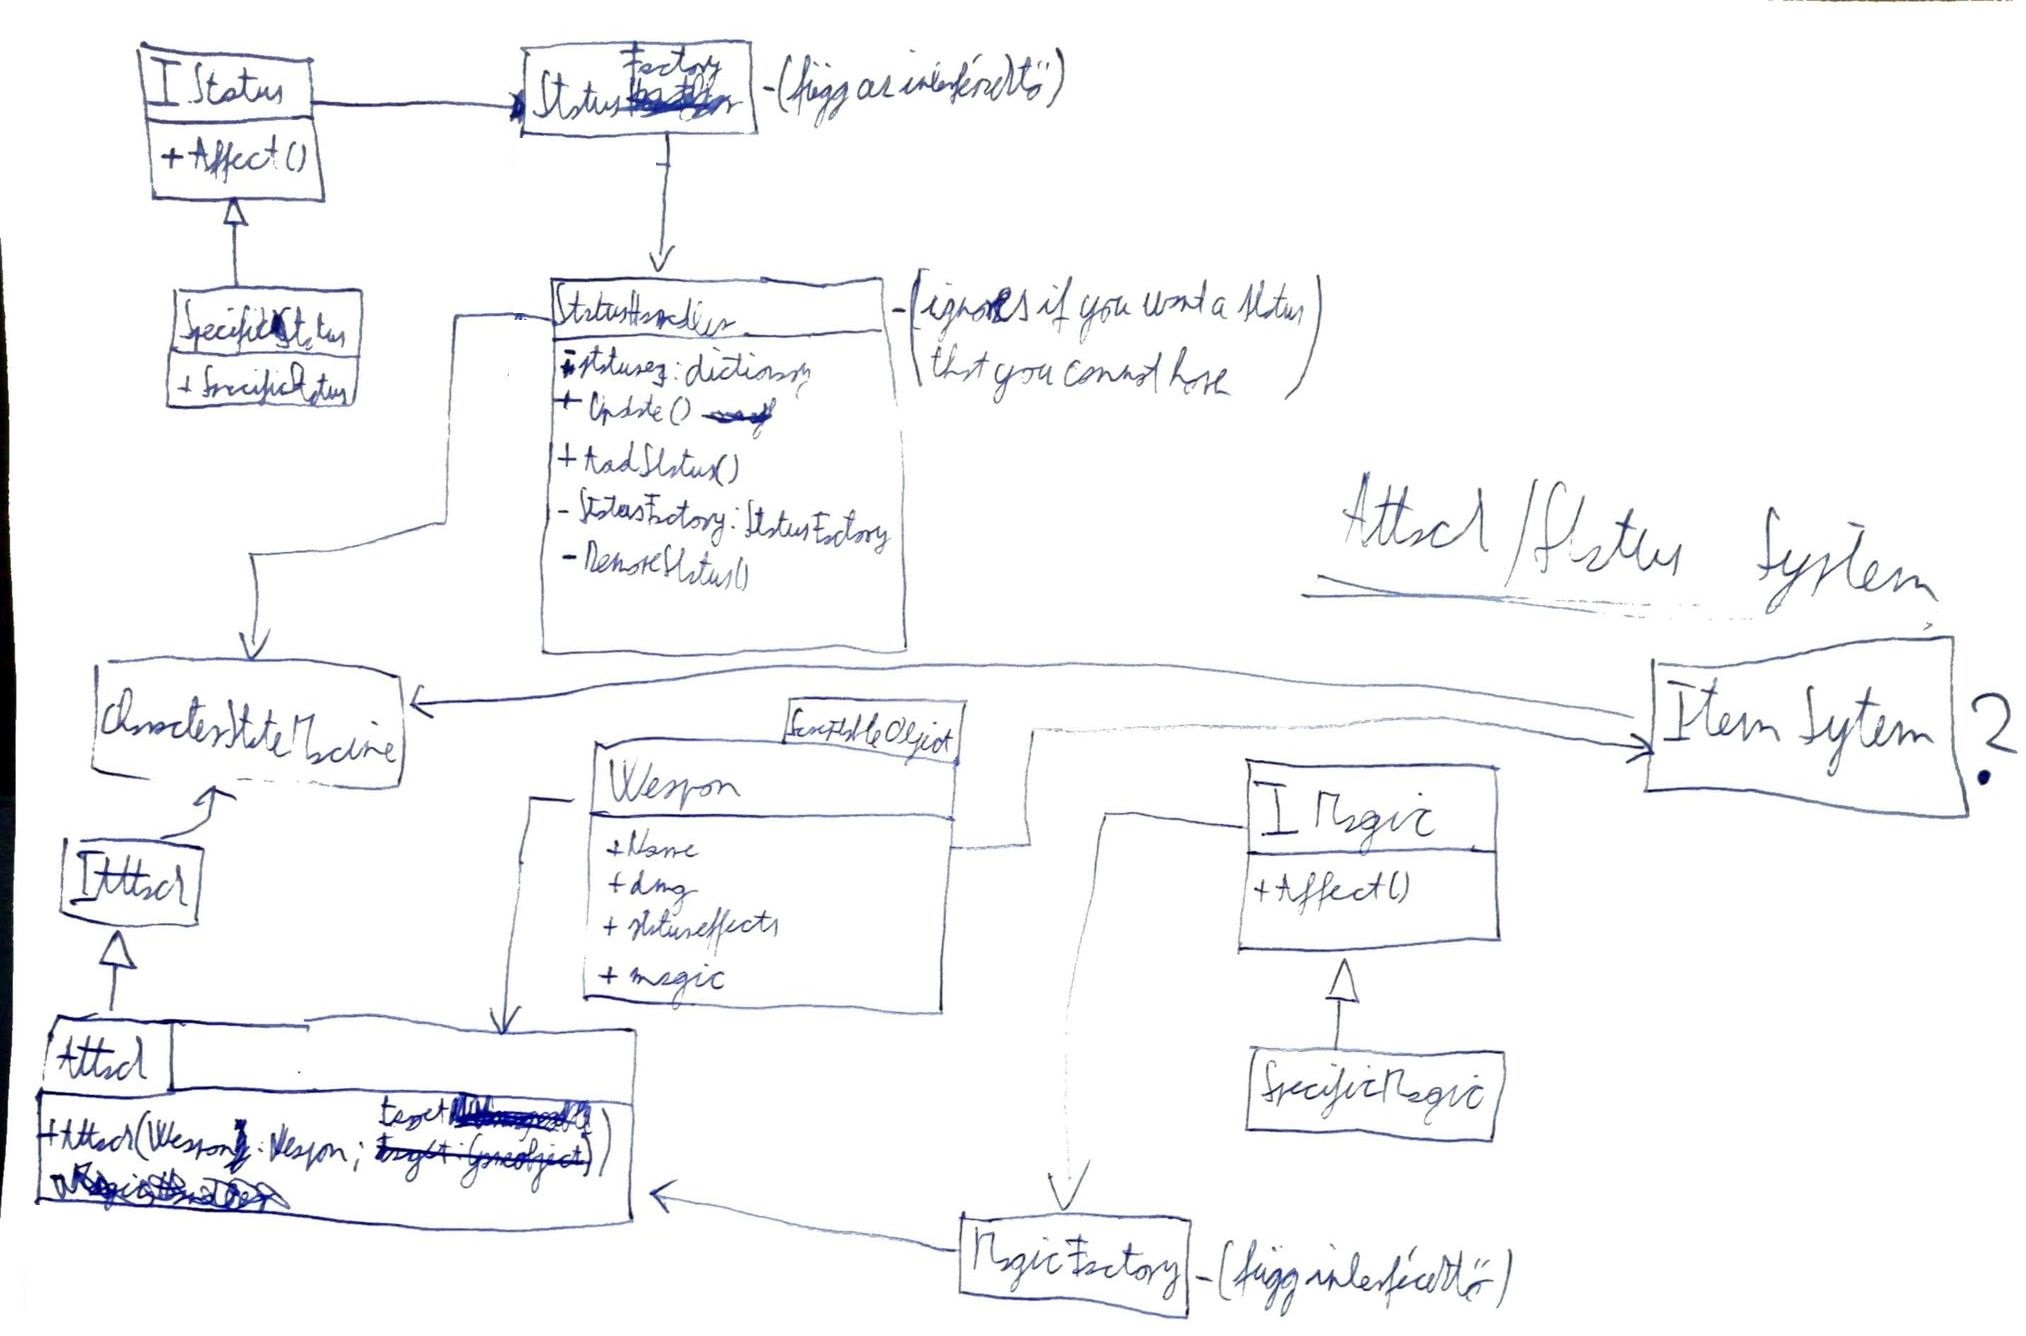
\includegraphics[width= 1\textwidth]{all}}
	\caption{Támadási rendszer}
	\label{all}
\end{figure}

\subsection{Unity}
A Unity játékmotor egy cross-platform komponens alapú játékfejlesztői motor. Ebben a fejlesztői környezetben, relatívan egyszerűen hozhatunk létre játékokat (főleg az új visual scripting segítségével, hiszen így fejlesztők nem kényszerülnek rá a C\# nyelv elsajátítására). Unity-ben 2 fontos dolgot kell megértenünk, egyik az Editor, amit használni fogunk a színterünk komponálására, valamit a komponenseink (GameObjects) létrehozására, a másik a monoBehaviour-ök megértése, hiszen ez az osztály az összes Unity script ősosztálya.\\
Először is a \textbf{Unity Editor}-ról beszélnék. Ez a Unity Engine gafikus interfésze, innen érhetjük el a Unity által biztosított funkciókat, mint például az \textit{animator}, ahol animációk átmeneteit határozhatjuk meg, a \textit{shader graph}-ot, ahol egy grafikus felületen készíthetünk vertex és fragment shader-eket, vagy akár a \textit{test runner}-t, hogy párat említsek.\\*
Azonban a 2 legfontosabb funkciója az Editornak a színtereink(scenes) és \textit{gameObject}-jeink komponálása. A színtereinken készíthetünk pályákat, menüket, adhatunk hozzá hangforrásokat, fényeket vagy utóhatásokat, nem mellesleg ide kell hozzáadnunk a gameObject-eket, hogy megjelenjenek.\\*
A \textit{gameObject}-ekteket el lehet képzelni úgy, mint egy üres dobozt,amihez különböző komponenseket adhatunk. Ha azt akarjuk, hogy ne láthatatlan legyen a dobozunk adhatunk hozzá egy \textit{Sprite Renderer}-t, ha akarjuk, hogy a fizika hasson rá akkor hozzáadhatjuk a \textit{Rigidbody} komponenst és így tovább. Egy gameObject rengeteg minden lehet és több funkciót is elláthat, nem mellesleg rájuk aggathatjuk a saját script-jeinket is, hogy valami egyedi hatást/viselkedést érjünk el.\\
Most, hogy beszéltem az Editor-ról, a helyről, ahol a játék építése folyik, beszélnék egy kicsit az egyik legfontosabb építőelemről, a \textbf{monoBehaviour}-ről, ami az összes script-ünk ősosztálya, amit egy \textit{gameObject}-re rá akarunk rakni, mint egy komponenst. A monoBehaviour és minden leszármazottja egy olyan osztály, amit nem lehet a \textbf{new} kulcsszóval példányosítani, csak az \textit{addComponent} függvénnyel. Ebből következve ezen osztályok, csak egy \textit{gameObject}-en élhetnek és kötöttek annak élettartalmához.\\*
A monoBehaviour biztosít számunkra pár fontos metódust is \cite{unityDocs}.
\begin{itemize}
	\item \textbf{Start} - inicializációs fázis utolsó lépése.
	\item \textbf{FixedUpdate} - fizikai frissítés. Itt lehet olyan fizikai számításokat kezelni, amiket minden ütemezett fizikai frissítésben végre akarunk hajtani.
	\item \textbf{OnCollisionXXX} - mi történjen ha valami ütközés történik.
	\item \textbf{Update} - elépzelhető mint egy monoBehaviour-re korlátozott \textit{gameLoop}. Akkor használjuk, ha ismétlődő számításokat akarunk végrehajtani (minden frame-ben).
\end{itemize}

\begin{figure}[H]
	\noindent\makebox[\textwidth]{
	\includegraphics[width= 1\textwidth]{thdfT}}
	\caption{MonoBehaviour életciklusa}
	\label{thdfT}
\end{figure}

\subsection{S.O.L.I.D.}
A S.O.L.I.D. elvek\cite{solid}

\textbf{S - Single-responsiblity Principle}, avagy az \textit{Egyetlen felelősség elve}\\
Ennek az elvnek a lényege, hogy egy osztálynak, egyetlen egy oka lehet a változásra, vagyis egy céljának kell lennie. Ennek az elvnek a megvalósítása Unity-ben triviális, hiszen kisebb odafigyeléssel ez adódik is a komponens alapú összetételből.

\textbf{O - Open-closed Principle}, avagy az \textit{Nyílt/zárt elv}\\
Itt a legfontosabb tudnivaló, hogy egy objektumnak képesnek (nyitottnak) kell lennie a bővítésekre, azonban ezeknek a bővítéseknek nem szabad módosítania a meglévő osztályt, zárva kell lennie a módosításokra tekintve. Ugye ez az elv interfészek és ősosztályok megvalósításával könnyen elérhető, hiszen ha megvannak a mintáink, hogy miképp kell egy osztálynak felépülnie, és azt meg is valósítottuk, esetleg egységtesztekkel le is védtük működését, akkor annak módosítása hiba nélkül nehéz lesz, azonban a bővítése triviális. Az a fontos itt, hogy a régi kódban lévő logika a bővítés miatt ne kényszerüljön az új kódrész függésére, ebben az esetben lehet érdemes meggondolni a kód feldarabolását a \textit{Egyetlen felelősség elve} mintájára.

\textbf{L - Liskov Substitution Principle}, avagy az \textit{Liskov helyettesítési elv}\\
Liskov helyettesítési elv lényege, hogy minden osztályt be kéne tudni helyettesíteni annak ősosztályába, interfészébe. Ez egy rendkívül fontos megállapítás, hiszen ezzel meg tudjuk szüntetni a függést egy specifikus osztályimplementációtól, ezáltal képesek leszünk könnyen cserélni konkrét működést egy komponensben/osztályban annak megváltoztatása nélkül.

\textbf{I - Interface Segregation Principle}, avagy az \textit{Interfész elválasztási elv}\\
Az elv azt mondja ki, hogy egy osztálynak nem szabad függenie olyan interfészektől, függvényektől, amiket nem valósít meg, nem használ. Ez könnyen felfogható, úgy mint az \textit{Egyetlen felelősség elve} alkalmazása interfészekre, hiszen így több kisebb közelebb kapcsolódó interfészt kapunk, amiket szabadon implementálhat egy osztály szükségszerűen, ellentétben egy nagy interfésszel.

\textbf{D - Dependency Inversion Principle}, avagy az \textit{Függőség megfordítási elv}\\
Ez az elv azt mondja ki, hogy az entitásoknak absztrakciókon kell függeniük, valamint, hogy magasabb rendű rendszereknek nem szabad függeniük az alacsonyrendűektől. Ezt a komponens alapú Unity-ben könnyen elérhetjük, hiszen ha osztályain egy interfészt implementálnak, ami megfelel az absztrakciónak és ezen osztályainkat a \textit{Liskov helyettesítési elv} és a \textit{Egyetlen felelősség elve} szerint hoztuk létre és mint Unity-s komponens használunk, akkor a magas szintű rendszereink tudnak csak az absztrakciótól függeni és Unity-ben intuitívan megvalósulni.

Mindezeket látva a Unity mint keretrendszer rendkívül alkalmas a S.O.L.I.D. elvek alkalmazására.

\subsection{Tervminták}
Miután átnéztük, hogy milyen elvek szerint lett elkészítve a játék, térjünk is át a szakdolgozat lényegére, a felhasznált tervmintákra és azok hasznára szerepére. A Game Programming Patterns-ben\cite{gameProgrammingPatterns} olvasott tervmintákat, néhány más hasznos mintával kiegészítve fogom kifejteni itt részletesebben, Jason Weimann\cite{jason} és DapperDino\cite{dapperDino} implementációit és példáit alapul véve. Ezek a minták kettő csoportba sorolhatók alapvetően, amik az \textbf{általunk implementált} tervezési minták és a \textbf{Unity/C\# által biztosított} tervezési minták, kezdjük is az utóbbikkal.

\textbf{Game Loop} - avagy a \textit{Játékciklus}\\
Ez a játék magja, legfontosabb alapköve. A Unity automatikusan biztosítja, nincs szükség egy komponáló osztályra, ahol egy while ciklusban hívódnának osztályaink. A tervminta lényege, hogy biztosítanunk kell egy a játék terminállásáig tartó folyamatos környezetet, ahol a játékos inputot, eseményeket és a játékon belüli időt kezelünk kell. Mivel ezt a modern játékfejlesztői környezetek alapértelmezetten tudják és elrejtik a felhasználó elöl (mint a Unity), ezért érdemes úgy tekinteni az ezen eszközökkel történő fejlesztés közben, mintha mindig a Játékciklusban lennénk.

\textbf{Update Method} - avagy a \textit{Frissítési metódus}\\
Ez a minta mögött az a gondolat húzódik, hogy vannak bizonyos számítások (például egy karakter pozícióváltozásából származó újrarajzolás) amiket minden egyes kirajzolt frame-ben végre szeretnénk hajtani. Unity-ben ezt a tervmintát még jobban felaprították, hiszen a monoBehaviour biztosít számunkra három különböző Update metódust is. A monoBehaviour életciklusa szerint \textit{FixedUpdate} amiben a fizikai számítások hajtódnak végre fix intervallumonként, \textit{Update}, ami egy általános frissítési metódus, itt végezzük a saját logikánk módosításainak nagyját, legvégül a \textit{LateUpdate}, ami egy a sima Update metódust, animáció frisítéseket és a coroutine-okat követő frissítés, ahol olyan operációkat hajthatunk végre, amiket az Update után szeretnénk végrehajtani.

\textbf{Component} - avagy a \textit{Komponens}\\
Ez a tervminta egy csoportosítási problémát szándékoz megoldani hasonlóan a Egyetlen felelősség elvéhez. Ezt a Unity szintén alapjaiban támogatja, hiszen az egész játékmotor komponens alapú (rigidbody, amiator, spriteRenderer, mint külön komponensek amiket egy gameObject-re tudunk ráaggatni, mint a saját script-jeinket).

\textbf{Type Object/Flyweight} - avagy a \textit{Típusobjektum/Pehelysúlyú}\\
Ezen tervezési minták, habár különböző, azonban egymáshoz rendkívüli módon kapcsolódó koncepciókat írnak le. A Típusobjektum lényege, hogy a példányspecifikus adatokat a típusolt objektumban tároljuk, míg az ezeket alkalmazó metódusokat/függvényeket, vagy közös adatokat a típusobjektumban definiáljuk, így a közös részeket és az egyedi adatokat elszeparáljuk. A Pehelysúlyú tervminta nagyon hasonlóan el akarja különíteni a példányspecifikus adatokat a megosztott minden azonos osztály számára szükséges és azonos adatoktól, ezáltal létrehozva egy pehelykönnyű osztályt. Mint láthattuk mindkettő tervminta célja a példányspecifikus adatok szeparálása, Unity-ben erre rendkívül jól használhatóak a \textit{ScriptableObject}-ek. Ezek egy különleges osztályok, amik többnyire adatstruktúrákat és közös működéseket írnak le. Miután definiáltunk egy ScriptableObject-et, azt legtöbbször nem a tradícionális módon kódból példányosítjuk, hanem a Unity Editor-ban hozzuk létre, mint új Asset-et, itt tudjuk az általunk megadott mezők értékeit kitölteni. Ha egy a ScriptableObject-et hozzárendelünk GameObject-ekhez akkor a különböző GameObject-ek között a ScriptableObject azonos marad, csak egyszer töltődik be a memóriába és minden változást az összes GameObject lát ha az adott ScriptableObject hozzá van rendelve.

\textbf{Prototype} - avagy a \textit{Prototípus}\\
A Prototípus minta lényege, hogy elkerüljük a felesleges alosztályok léterehozását azzal, hogy létrehozunk, egy prototípus osztályt, ami klónozással hoz létre új példányokat. Unity-ben ez a \textbf{prefab}-ekkel van megoldva. A prefab-ek egy asset-ként elmentett elemek, amit az editoron keresztül tudunk módosítani tetszés szerint, majd példányosítani azt. 

\textbf{Observer} - avagy a \textit{Figyelő}\\
Ez a tervminta annyira elterjedt, hogy a C\# nyelvbe natívan támogatva is van az eseményrendszeren keresztül. Unity-ben is támogatva van a C\#-os eseményrendszer, azonban a Unity-biztosít egy saját eseménykezelést is ez nem más mint a \textit{Unity event}-ek. Ezek lényegében egy kényelmi funkciót látnak el, hogy egyszerűen tudjunk az Editor-ban összekötni eseményeket, ezen események általában olyan elemek, amit kóddal ritkán váltunk ki (általában UI gombnyomások vagy az Input System-ből érkező események), azonban saját funkciót szeretnénk kötni különösebb komplikáció nélkül.

\textbf{Object Pool/Object Pooling} - avagy az \textit{Objektumkészlet}\\
Az Objektumkészlet tervezési minta mögötti elv, a memória használat csökkentése és a teljesítmény növelése. Ezt azzal érjük el, hogy az objektumainkat, nem mindig újonnan hozzuk létre, hanem  egy előre legyártott készletből kérünk egy elemet, és mikor erre az elemre már nincs szükségünk, akkor ez visszakerül a készletbe. Ez egy játékba különösen fontos, hiszen egy objektum létrehozása költséges művelet. Unity-ben, ami ugye egy C\# alapú játékmotor, nem is feltétlen a példányosításnál látjuk a problémákat, hanem, mikor a Garbage Collector lefut és felszabadítja a nem használt erőforrásokat. Ilyen esetekben nagy a valószínűsége a frame rate bezuhanásának, ami rossz felhasználói élményhez vezet. Erre tökéletes megoldást jelent az Objektumkészlet, hiszen, ha nincs megszűnt objektum, akkor nincs Garbage Collection sem.

\textbf{Command} - avagy a \textit{Parancs}\\
A Command pattern lényegében egy callback objektumorientált megfelelője, vagyis használhatunk vele objektumokat arra, hogy más rendszerek/objektumok mit csináljanak. A játékfejlesztésben ez rengeteg helyen hasznosítható. Egyszerűen lehet a parancs tervmintával játékos bemeneteket, kezelni, és akár visszavonni azokat, vagy akár egy játékon belüli boltban a vétel is lehet egy parancs és, ha meggondolunk magunkat, akkor a vétel parancs undo metódusával visszacsinálhatjuk a tranzakciónkat, csak hogy egy konkrétabb példával éljek.

\textbf{Singleton} - avagy az \textit{Egyke}\\
Az egyke tervezési minta, egy egyszerű elven alapszik, biztosítsuk, hogy egy osztálynak, csak egy globálisan elérhető példánya legyen. Ez bizonyos rendszereknél, például mentési rendszer, scene menedzser rendszer, hangkezelő rendszer. Ezen rendszerekben közös, hogy ha több lenne belőlük, akkor az problémákhoz vezethet (csak egy példány legyen), elérni nem feltétlenül egy helyen szeretnénk őket (legyenek globálisok), szóval láthatjuk miért hasznos ilyen esetekben ha ezen osztályaink/rendszereink egykék lennének. Azonban a singleton tervminta túlhasználtsága, architekturális problémákhoz vezethet. Hiszen a bonyolultabb tervezést megkerülve könnyen elérhető, azonban globális struktúrákat definiálhatunk, amik problémákhoz vezethet, például ha publikusan elérhető akárki által változtatható adatokat tárolunk egy egyke osztályban, az könnyen látható, hogy problémákhoz vezethet. Azonban talán az egyik legnagyobb hátrányuk az egyke osztályoknak, hogy egységtesztelhetőségük nehézkes, különösen Unity-ben ahol ezen osztályok gyakran MonoBehaviour-ök is, amik tesztelése rendkívül körülményes.

\textbf{Humble Object} - avagy a \textit{Szerény Objektum}\\
A Szerény Objektum, Unity-ben egy kimagaslóan hasznos tervezési minta, hiszen az a lényege, hogy egy bonyolultabb objektumból, ami több nehezen tesztelhető függőséggel rendelkezik (például a MonoBehaviour, aminek tesztelése sok felesleges előkészülettel jár), kiemeljük a tesztelni kívánt logikát, olyan szinten, hogy az így keletkezett Szerény Objektumot, már ne kelljen tesztelni. Az így kapott logikai osztály már csak minimális függőségekkel kell rendelkeznie és már (egység) tesztelni egyszerű.

\textbf{Factory} - avagy a \textit{Gyártó}\\
A gyártó minta célja, hogy átadjuk az példánykészítés folyamatát egy erre speciálisan kitalált osztálynak. Ennek az az értelme, hogy nem keletkeznek elszórt példányosítások, amiknek a módosítása egyesével bonyodalmas és problémákat vethet fel. Ehelyett a példányaink egy helyről származnak, ha valahogy módosítani szeretnénk létrejöttjüket, azt egy helyen meg tudjuk tenni. Ennek a mintának az előnye a játékfejlesztésben nagyon hamar elő tud jönni, hiszen a játékokban, gyakran vannak különböző tárgyak, varázslatok, effektusok, akár ellenségek, amiket dinamikusan akarunk létrehozni és egy központi gyártó osztállyal mindezt strukturáltabban el tudjuk érni.

\textbf{State/State machine} - avagy a \textit{Állapot/Állapotgép}\\
Ennek a mintának a játékfejlesztésre vetített lényege, hogy a játék, ne kerülhessen olyan állapotba, amibe nem szabadna, neki. Az állapot tervezési minta, megfogalmaz a nevéből eredően állapotokat, a köztük lévő átmentetek és azok feltételeit, valamint az egész rendszert összekötő állapotgépet. Ez több szempontból is hasznos, egy játékos karaktere komplex viselkedéssel bír, éppen ezért fontos, hogy ne lehessen kódolási hibából nem megengedett állapotba lépni (például, ha ugrani csak akkor lehet, ha a földön vagyunk, akkor ne lehessen a levegőbe ugrani). A játékoskarakter állapotainak és a köztük lévő kapcsolatok leírásával, tehát egy álltopgéppel tiszta architektúrával le tudjuk írni, elkerülve a végtelenségig nyúló if-else és switch elágazásokat. Egy karakterkontrolleren kívül azonban használható önállóbb rendszerekre is az állapotgép, például ellenségek/játékon belüli objektumok viselkedésének (pszeudo AI) leírására is. A Unity-ben az animációk kapcsolata, egy grafikus állapotgépen keresztül van definiálva.

\cleardoublepage
\section{Megvalósítás}
A megvalósítás során látható, hogy alkalmaztam a Szerény objektum tervezési mintát a legtöbb helyen. A logikai részeket (move, attack, inventory) kiemeltem egy osztályba, amiket egy Unity-s MonoBehaviour osztály csomagol be, hogy az Editor-ban ezeket a komponenseket, csak rá kelljen "húzni" arra az objektumra, aminek szüksége van rá (természetesen, ahol lehetett az osztályok az interfészeiken keresztül hivatkoznak egymásra). Az így készült komponens alapú megközelítés nagy személyre szabhatóságot biztosít, hiszen ha készítünk, teszem azt egy új bolt komponenst, ahol lehet vásárolnunk, akkor csak rá kell húznunk arra az objektumra amelyiken szeretnénk, hogy elérhető legyen ez a funkció, az interfészeken keresztül történő elérés, pedig biztosítja, hogy a különböző megvalósítások nem okoznak problémát.

\begin{figure}[H]
	\noindent\makebox[\textwidth]{
	\includegraphics[width= 1.1\textwidth]{GeneralComponentSystem}}
	\caption{Általános komponens kapcsolat}
	\label{GeneralComponentSystem}
\end{figure}

\subsection{Felhasználói esetdiagram} 
\begin{figure}[H]
	\noindent\makebox[\textwidth]{
	\includegraphics[width= 1.15\textwidth]{useCase}}
	\caption{Felhasználói eset diagram}
	\label{useCase}
\end{figure}

\subsection{Státusz rendszer}
A státusz rendszer a második legbonyolultabb rendszer a játékos rendszer után. A lényege, hogy a \textit{StatusHandler} osztály lekezeli az aktív státuszokat, az újakat el cache-eli, hogy ne kelljen a költséges statikus gyártóosztályt hívogatni potenciálisan frame-enként. A \textit{StatusFactory} osztály reflekcióval megtalálja az összes \textit{StatusBase} leszármazottat, hogy abból példányt tudjon szolgáltatni, a \textit{StatusFactory} számára. A \textit{StatusBase} minden specifikus státusz ősosztálya. Egy-egy specifikus osztály merőben különböző hatásokat válthat ki, azonban  mindegyik fog hatni valamilyen módon bizonyos időintervallumonként. Lehet előhatása, ahol eltárolhat szükséges adatokat és módosíthat más rendszerekben paramétereket, lehet utóhatása, ahol visszaállíthatja az elmentett állapotot, jelezve a státusz hatásának végét. A különböző funkciókhoz szükséges függőséginjektálást a \textit{GetComponent} függvénnyel szerzi meg. Egy \textit{StatusHandler}-t a \textit{StatusHandlerComponent} burkolja, amit hozzátudunk adni objektumokhoz, ha szeretnénk, hogy a státuszok hassanak rájuk.

\begin{figure}[H]
	\noindent\makebox[\textwidth]{
	\includegraphics[width= 1.1\textwidth]{StatusSystem}}
	\caption{Státusz rendszer UML}
	\label{StatusSystem}
\end{figure}

\subsection{Varázslás rendszer}
A varázslatok rendszere strukturálisan, nagyban hasonlít a státuszok rendszerére. A nagy különbség, hogy a specifikus varázsaltok, nem automatikusan, hanem egy támadás keretén belül vannak aktiválva és a \textit{Use} metódusuk sokkal komplexebb logikát tartalmaz, mint egy státusz. \textit{MagicHandler} itt is eltárolja a használt varázslatot. A specifikus varázslatok használatát a \textit{UseMagic} metóduson érhetjük el. Itt is mint a státusz rendszernél, egy komponensbe van beburkolva a \textit{MagicHandler} és ezt a komponenset azokra az osztályokra rakjuk rá, amiket szeretnénk, hogy varázslatot tudjon használni, fontos, hogy nem azokra, amikre szeretnénk, hogy egy varázslat hasson.

\begin{figure}[H]
	\noindent\makebox[\textwidth]{
	\includegraphics[width= 1\textwidth]{MagicSystem}}
	\caption{Varázslat rendszer UML}
	\label{MagicSystem}
\end{figure}

\subsection{Játékos rendszer}
A játékos rendszer a legbonyolultabb rendszer a szakdolgozatomba. \textit{PlayerStateMachine} osztályban vannak definiálva a játékoskarakter fontos metódusai (Respawn, Dead, Load), valamint itt helyezkedik el maga az állapotgép is. Itt található az állapotok közti átmentek és azok feltételei is, valamint az állapotokhoz szükséges dependenciák. Az \textit{InputController} osztályban találhatók azok a metódusok, amiket a Játékos bemenetekből érkező események hívnak, valamint ezek időfeltétele. Ez az osztály felel az állapotváltozók beállításáért, amiken az állapotok átmenetfeltételei alapszanak.

\begin{figure}[H]
	\noindent\makebox[\textwidth]{
	\includegraphics[width= 1\textwidth]{PlayerSystem1}}
	\caption{Játékos főosztály UML}
	\label{PlayerSystem1}
\end{figure}

Azonban ennek a rendszernek a legfontosabb eleme az állapotok. Ezek nélkül nem lehetne a játékoskaraktert irányítani.\\*
Az alapértelmezett állapot az \textbf{Idle} állapot, ez egy "üres" helyzet, amikor a játékos egy helybe áll.\\*
A \textbf{Move} állapot lehetővé teszi a jobb és a bal irányú mozgást, valamint a "dash" műveletet és elindítja a futásanimációt.\\*
A \textbf{Jump} állapot lehetővé teszi, hogy ugorjunk és közben horizontálisan mozogjunk, vagy dash-eljünk, valamint elindítja az ugrás animációt.\\*
A \textbf{Fall} állapotba akkor érkezünk, ha ugrás után lefele ívelő lesz a mozgásunk, vagyis akkor, ha elfogy az ugrásból érkező lendületünk. Miután ebbe az állapotba érünk a normális gravitációnál egy kicsit gyorsabban kezdünk zuhanni, ezáltal a már más játékokból megszokott hatást keltve. Mindezen kívül az állapot elkezdi játszani a zuhanás animációt.\\*
A \textbf{PushBack} állapotba akkor érkezünk, ha egy ellenségbe ütközünk, ekkor hátralök minket a játék, és lejátssza a hátralökődés animációt.\\*
A \textbf{Attack} állapot lehetővé teszi, az aktuális felhasználói bemenettől függően, az eszközeink használatát és a hozzájuk illő animáció lejátszását.\\*
A \textbf{Death} állapot megkezdi a játékos újraéledési procedúráját és lejátssza a halott animációt.\\
Mint látható az összes a menürendszeren kívüli felhasználói interakció a játékoskarakter állapotgépén keresztül történik, aminek a belépőpontja a \textit{PlayerStateMachine} osztály, aminek komplexitása emiatt érthető. Az is látszik, hogyha nem egy állapotgép lenne a karakterkontroller, hanem egy egyszerű osztály, akkor annak komplexitása és átláthatósága is megnőne, hiszen egyszerre kéne ellátnia az állapotok és az azokat menedzselő osztály feladatát.

\begin{figure}[H]
	\noindent\makebox[\textwidth]{
	\includegraphics[width= 0.75\textwidth]{PlayerSystem2}}
	\caption{Játékos állapotok UML}
	\label{PlayerSystem2}
\end{figure}

\subsection{Ellenség rendszer}
Az ellenségek rendszere a játékos rendszerének egy leegyszerűsítése. A játékos rendszerből a felhasználói bemenet kivételével és a játékoskarakterre specifikus metódusok eltávolításával és egy kevés ellenség specifikus kóddal meg is kapjuk, az ellenség rendszert. A legnagyobb kettő különbség, az ellenség specifikus állapotok és a játékos megtalálására/érékelésére felállított rendszer.\\*
A \textit{TargetSetter} osztály felel azért, hogyha a játékos látótávolságon belül van egy ellenséghez képest, akkor az az ellenség erről tudjon és a megfelelő állapotba lépjen. A \textit{InRange} osztály felel azért, hogy ha a játékos elég közel van egy ellenséghez, akkor az ellenség a támadás állapotába (Attack) lépjen.

\begin{figure}[H]
	\noindent\makebox[\textwidth]{
	\includegraphics[width= 0.8\textwidth]{EnemySystem}}
	\caption{Ellenség rendszer UML}
	\label{EnemySystem}
\end{figure}

A \textbf{MoveTo} állpotban kezd el az ellenség a játékos felé mozogni. A \textbf{Patrol} állapotban a \textit{PatrolEnemy} elkezd kettő pont között mozogni az \textit{Idle} állapot helyett.

\subsection{Adattárolás}
Az adatok tárolására kettő megoldást használtam. Az egyszerűbb adatokra, mint például a játékos neve és a beállítások, a Unity által biztosított plyerPrefs-et használtam, ami a registry-be menti az adatokat. A bonyolultabb és nagyobb adatok mentésére (eredménytábla, játékosmentés) egy binaryFormatter-t használtam, ami a \textit{SaveSystem} osztályban található, ehhez a menteni kívánt adatokra létrehoztam szerializált osztályokat \textit{(ScoreData, SaveData)}.\\*
Windows-on a \textit{\textbackslash AppDat\textbackslash LocalLow\textbackslash HMF\textbackslash The Quest for the Thesis} elérési úton találhatóak a mentések,\\
Linux-on a \textit{/.config/unity3d} vagy a \textit{/unity3d} elérési úton.\\
A \textit{SavePlayer} osztály felelős a mentési rendszert összekötni a játék többi rendszerével (GUI, játékoskarakter).\\
A \textit{PersistentData} osztály felelős a betöltött adatok átjuttatásához különböző scene-ek között. Ez az osztály egy egyke osztály, hiszen olyan adatokat tartalmaz, amiket globálisan elszeretnénk érni, azonban ha több példánya lenne, akkor nem lehetne követni, hogy melyikek a nekünk megfelelő betöltött adatok, ezeket látva döntöttem az egykesége felől.

\begin{figure}[H]
	\noindent\makebox[\textwidth]{
	\includegraphics[width= 1\textwidth]{SaveSystem}}
	\caption{Mentés rendszer UML}
	\label{SaveSystem}
\end{figure}

\cleardoublepage
\subsection{CI/CD pipeline}
A szakdolgozatom verziókezelésére github-ot használtam. A github actions segítségével építettem ki a CI/CD folyamatomat. Először is, ha a fejlesztői ágra beérkezik egy új commit, vagy egy új pull request, akkor lefut a teszt folyamat. Ez a folyamat végrehajtja az egységteszteket, majd ha sikereske voltak a teszek készít egy code coverage jelentést.

\begin{figure}[H]
	\noindent\makebox[\textwidth]{
	\includegraphics[width= 1\textwidth]{codeCoverage}}
	\caption{A Logic assembly tesztelési lefedettsége}
	\label{codeCoverage}
\end{figure}

Ha a main ágra érkezik egy új pull request, akkor ugyanúgy lefut a tesztelési folyamat és a code coverage jelentés generálása, azonban ha sikeres volt a teszt, akkor megkezdődik a build folyamat. Ez elkészíti a kívánt (előre beégettet) platformra a lefordított, futtatható játékot. Mindez után, ha sikeres volt a build folyamat, akkor elkészíti az automatikus dokumentációt és kitelepíti azt a \textit{\url{https://thesis-docs.netlify.app}} címre.

\cleardoublepage
\section{Tesztelés}

\subsection{Egységtesztek}
Az egységtesztelést white box módon hajtottam végre. A Unity biztosít kettőféle tesztelési környezetet, Editor mode és Play mode. Én a Play mode-ot használtam, ami a játékban futtatja a teszteket, nem az editorban. A Szerény objektum (Humble Object) segítségével kiemelt logikai osztályaimat teszteltem. A teszteléshez NUnit keretrendszert használtam, mock-oláshoz pedig a Moq egy Unity kompatibilis verzióját.

\begin{figure}[H]
	\noindent\makebox[\textwidth]{
	\includegraphics[width= 0.55\textwidth]{tests}}
	\caption{Az egységtesztek eredményei}
	\label{tests}
\end{figure}

\subsection{Kézi Tesztelés}

\begin{center}
	\begin{longtable}{| m{0.4\textwidth} | m{0.4\textwidth} | m{0.2\textwidth}|} 
		\hline
		\textbf{Helyzet} & \textbf{Elvárás} & \textbf{Státusz}\\ \hline \hline
		
		Játék indítása & Játék elindul & Sikeres\\ \hline
		
		Főmenüben Scoreboard gombra kattintás & Megjelenik az eredménytábla & Sikeres\\ \hline
		
		Eredménytáblánál a Back gombra kattintás & Visszatérünk a főmenübe & Sikeres\\ \hline
		
		Főmenüben Scoreboard gombra kattintás & Megjelenik a köszönetnyilvánítás & Sikeres\\ \hline
		
		Köszönetnyilvánításnál Back gombra kattintás & Visszatérünk a főmenübe & Sikeres\\ \hline
		
		Főmenüben Exit gombra kattintás & Játék bezáródik & Sikeres\\ \hline
		
		Főmenüben Settings gombra kattintás &  Megjelennek a beállítások & Sikeres\\ \hline
		
		Beállítások változtatása & Azonnali beállításváltás & Sikeres\\ \hline
		
		Beállításoknál Back gombra kattintás & Visszatérünk a főmenübe & Sikeres\\ \hline
		
		Főmenüben Settings gombra kattintás újra &  Megjelennek a megváltoztatott beállítások & Sikeres\\ \hline
		
		Főmenüben Start gombra kattintás & Megjelenik a pályaválasztó & Sikeres\\ \hline
			
		Pályaválasztóban Name mezőbe írás & Megváltozik a nevünk & Sikeres\\ \hline
		
		Pályaválasztóban Load gombra kattintás & Megjelennek a mentések & Sikeres\\ \hline
		
		Mentéseknél egy mentett állapotra kattintás & Kijelöljük az állapotot & Sikeres\\ \hline
		
		Pályaválasztóban Load gombra kattintás & Betölt a mentet állás az instrukció menüvel & Sikeres\\ \hline
		
		Pályaválasztóban Back gombra kattintás & Visszatérünk a fő menübe & Sikeres\\ \hline
		
		Pályaválasztóban az egyik pályára gombra kattintás & Betölt a pálya az instrukciómenüvel & Sikeres\\ \hline
		
		Instrukciómenüben a Play gombra kattintás & Elkezdődik a játék & Sikeres\\ \hline
		
		A játékban ESC megnyomása & Megjelenik a szünet menü & Sikeres\\ \hline
		
		Szünetmenüben Resume gomb megnyomása & Játék folytatása & Sikeres\\ \hline
		
		Szünetmenüben Save/Load gomb megnyomása & Megjelennek a mentések & Sikeres\\ \hline
		
		Mentésmenüben egy hely kiválasztása után Save gomb megnyomása & A jelenlegi állás elmentődik & Sikeres\\ \hline
		
		A játékban A/D megnyomása & Mozgás jobbra/balra & Sikeres\\ \hline
		
		A játékban SPACE megnyomása & Ugrás & Sikeres\\ \hline
		
		A játékban Bal ALT megnyomása & Gyors hirtelen mozgás & Sikeres\\ \hline
		
		A játékban bal egérgomb megnyomása & Sima támadás & Sikeres\\ \hline
		
		A játékban 1,2,3,4 megnyomása & Megfelelő eszköz használata, cooldown megjelenítése & Sikeres\\ \hline
		
		A játékban ellenség közelébe menés & Ellenség jön felénk és támad & Sikeres\\ \hline
		
		A játékban nullára megy az életünk & Újraéledés & Sikeres\\ \hline
		
		A játékban ellenséget sokszor támadjuk & Ellenség meghal & Sikeres\\ \hline
		
		A játékban ellenség státuszeffektust rak ránk & Megjelenik a státuszeffektus bal felül & Sikeres\\ \hline
		
		A játékban státuszeffektus rajtunk van & Hat a státusz & Sikeres\\ \hline
		
		A játékban elmúlik a státuszeffektus & Eltűnik felülről a státusz & Sikeres\\ \hline
		
		A játékban elérünk a pálya végére & Megjelenik a vége menü & Sikeres\\ \hline
		
		A vége menüben & Megjelenik a pontunk és a többi pálya amire léphetünk & Sikeres\\ \hline
		
	\end{longtable}
\end{center}

\subsection{Tesztelési konklúzió}

Az egységtesztek miatt ha módosítani is kellett a logikai osztályokat, akkor is az elvárt viselkedést mutatták, vagy ha nem akkor az hamar és pontosan kiderült, ezzel időt spórolva a hibakeresés során. Az egységtesztek írása során továbbá sikerült olyan hibákat találni, amikre, ha manuális tesztelés során találtam volna rá, sokkal több munka árán tudtam volna javítani.\\
A manuális tesztek segítették a rendszerek közötti kapcsolatok és az általános játékmenet tesztelését és finomítását. Összegezve a tesztek nélkül egyértelműen több időt vett volna igénybe a szakdolgozatom elkészítése, és lényegesen alacsonyabb minőségű szoftver keletkezett volna.